    %%%%%%%%%%%%%%%%%%%% CHAPTER  %%%%%%%%%%%%%%%%%%%%%%%
    %------------------------------------- Preeliminares-------
    \chapter{Preliminares}
    Antes de poder hablar del Aprendizaje profundo, o de Redes Neuronales Convolucionales, es importante sentar las bases matemáticas y computacionales requeridas para su estudio. A continuación, se presentan algunas definiciones y resultados conocidos de temas tales como Cálculo, Álgebra y Ciencias de la Computación.
    \section{Resultados de Cálculo y Álgebra lineal}
    \begin{definition}
        Sean $A$ y $B$ dos conjuntos. El producto cartesiano $A \times B$ se define como
        \begin{eqnarray}
            A \times B &:= \{(a,b) : a\in A \text{ y } b\in B\}.
        \end{eqnarray}
        De igual manera sean $A_1, ..., A_s$ son conjuntos, el producto cartesiano se define como
        \begin{equation}
            A_1\times A_2 \times ... \times A_s = \{(a_1,..., a_s): a_i\in A_i, \quad i= 1,...,s\}.
        \end{equation}
        De modo natural, se define $A^n :=  A \times A \times ... \times A$ donde $A$ se repite $n$ veces.
    \end{definition}
    A su vez, es conveniente destacar otra notación
    
    \begin{notation}
        Sean $a_1, ..., a_n\in \mathbb N$. Denotamos $\mathbb R^{a_1 \times a_2 \times ... \times a_s} := \mathbb R^{a_1} \times ... \times \mathbb R^{a_s}$.
    \end{notation}

    \begin{definition}
        Sean $u,v\in \mathbb R^n$, el producto punto de $u$ con $v$ denotado como $u\cdot v$ es
        \begin{equation}
            u_1v_1 + u_2v_2 + ... + u_nv_n,
        \end{equation}
        donde $u_i$ y $v_i$ representan la $i$-ésima entrada de los vectores $u$ y $v$ respectivamente.
    \end{definition}
    \begin{definition}[Polinomio de Taylor]
        Sea $f$ una función $n$ veces diferenciable, y sea $$a_k = \frac{f^{(k)}(a)}{k!}.$$
        Se define el Polinomio de Taylor de grado $n$ para $f$ en $a$ como
        $$P_{n,a}(x) = a_0 + a_1(x-a) + \cdots + a_n(x-a)^n.$$
        dónde $f^{(k)}$ representa la k-ésima derivada de $f$.
    \end{definition}
    El polinomio $P_{n,a}(x)$ ha sido definido de manera que $P_{n,a}(a) = f(a)$ para $0\leq k \leq n$.
    \begin{definition}
        Sea $f$ una función tal que $P_{n,a}(x)$ existe, definimos el término  residual $R_{n,a}(x)$ como 
        \begin{equation}
            R_{n,a}(x) = f(x) - P_{n,a}(x).
        \end{equation} 
    \end{definition}
    \begin{theorem}[Teorema de Taylor]
        Supóngase que $f^{(1)}$, $f^{(2)}$, ..., $f^{(n+1)}$ están definidos en $[a,x]$. Entonces 
        \begin{equation}
            R_{n,a}(x) = \frac{f^{(n+1)}(t)}{(n+1)!}(x-a)^{n+1}
        \end{equation}
        para algún $t\in (a,x)$.
    \end{theorem}
    Para clasificar las imágenes, los algoritmos de inteligencia artificial extraen \textsl{características} importantes de una imagen. ¿Qué puede ser tomado en cuenta como importante? Podría pensarse que las esquinas, los bordes u otros detalles. Sin embargo, los algoritmos de aprenizaje automático suelen ser tomadas como cajas negras, dónde las caraceterísticas relevantes de una imagen, a simple vista no parezcan intuitivas bajo la percepcion humana.
    \begin{definition}[Característica]
        Una característica $x$ es un elemento de $\mathbb R^{w\times h\times d}$, dónde $w,h\in \mathbb N$ representan las dimensiones espaciales y $d$ la cantidad de canales.
    \end{definition} 
    
    \begin{figure}[H]
        \centering
        \includegraphics[width=6in]{../cap1_preliminares/src/features.jpg}
        \caption{En las redes neuronales convolucionales, las imágenes pasan por múltiples filtros. El resultado de cada convolución, es una característica.} 
    \end{figure}

    \begin{definition}
        Sea $x$ una característica en $\mathbb R^{h\times w\times d}$. La vectorización de $x$, denotada $X = \vect(x)$ es un vector en $\mathbb R^{hwd}$ tal que 
        \begin{equation}
            X_{(k-1)hw + (i-1)w + j} = x_{i,j,k},
        \end{equation}
        para todos $i=1,2, ..., h$, $j = 1, 2, ..., w$, $k= 1,2,..., d$.
    \end{definition}
    \begin{definition}
        Una matriz $H$ es llamada \textsl{Circulante} si es de la forma
        \begin{equation}
            H = \begin{bmatrix}
                h_0 & h_1 & \cdots & h_{N-1} \\
                h_{N-1} & h_0 & \cdots & h_{N-2} \\
                \vdots & \vdots &  & \vdots \\
                h_1 & h_2 & \cdots & h_{0} \\
            \end{bmatrix}
        \end{equation}
        ya que $H$ queda completamente determinada con la primera fila, es posible escribir $H = \text{circ}(h_0, ..., h_{N-1})$.
    \end{definition} 
    \begin{definition}
        \label{doubly_circulant_matrix}
        Una matriz $H$ es llamada \textsl{Doblemente Circulante por Bloques} si es de la forma
        \begin{equation}
            H = \begin{bmatrix}
                H_0 & H_1 & \cdots & H_{N-1} \\
                H_{N-1} & H_0 & \cdots & H_{N-2} \\
                \vdots & \vdots &  & \vdots \\
                H_1 & H_2 & \cdots & H_{0} \\
            \end{bmatrix} = \text{circ}(H_0, ..., H_{N-1}) \in \mathbb R^{N^2\times N^2}
        \end{equation}
        dónde $H_i = \text{circ}(h_{i,0}, ..., h_{i, N-1}) \in \mathbb R^{N \times N}$.
    \end{definition}

    \begin{definition}
        Una función vectorial es una función de la forma $f:\mathbb R \to \mathbb R^n$.
    \end{definition}

    \begin{definition}
        La derivada $f'$ de una función vectorial $f: \mathbb R \to \mathbb R^n$ se define como
        \begin{equation}
            f'(t) = \lim_{h\to 0} \frac{f(t+h)- f(t)}{h}.
        \end{equation}
    \end{definition}
    Un teorema útil para encontrar derivadas vectoriales es el siguiente:
    \begin{theorem}
        La derivada $f'$ de una función vectorial $f = (f_1, f_2, ..., f_n)$, con $f_i: \mathbb R \to \mathbb R$ está dada por
        \begin{equation}
            f'(t) = (f_1'(t), f_2'(t), ..., f_n'(t)).
        \end{equation}
    \end{theorem}
    \begin{definition}[Gradiente]
        Sea $f: \mathbb R^n \to \mathbb R$. El gradiente de $f$ es el vector conformado por las derivadas parciales en cada una de las $n$ variables:
        \begin{equation}
            \nabla f = \left(\frac{\partial f}{\partial x_1}, ..., \frac{\partial f}{\partial x_n}\right).
        \end{equation}
    \end{definition}
    \begin{proposition}[Regla de la cadena]
        Sea $f: \mathbb R^n \to \mathbb R$ y $v: \mathbb R \to \mathbb R^n$. Es posible hallar la derivada de la composición.
        \begin{equation}
            \frac{d}{dt}(f\circ v) = \nabla f(v(t)) \cdot  v'(t)
        \end{equation}
    \end{proposition}

    \begin{definition}[Notación O-grande (Big O)]
        Sean $f$ y $g$ funciones $f,g:\mathbb N \to \mathbb R^+$. Decimos que $f(n) = \mathcal O(g(n))$ si existen enteros positivos $c$ y $n_0$ tales que para cualquier entero $n\geq n_0$,
        \begin{equation}
            f(n) \leq cg(n).
        \end{equation}
        Cuando $f(n) = \mathcal O(n)$, decimos que $g(n)$ es una cota asintótica superior de $f(n)$.
    \end{definition}

    %------------------------------------- Vision computacional -------
    \section{Visión Computacional}
    El problema d e clasificación de imágenes, pertenece a la rama de la visión computacional. La siguiente definición de imagen fue extraída del libro \cite{computer_vision}.
    \begin{definition}
        \label{digital_image}
        Una \textsl{imagen digital} es una función $I:  D \subset \mathbb Z^2 \to U$. Dónde el domino es un rectángulo con coordenadas enteras $D = [1,M]\cap \mathbb Z \times [1,N] \cap \mathbb Z$. La terna $(x,y,u)$ se conoce como pixel.
        \begin{itemize}
            \item Cuando las imágenes son a escala de grises se tiene que $U=[0,255]\cap \mathbb Z$. Es decir que $u\in U$ es un valor de 0 a 255.
            \item Si las imágenes son a color, consideramos $U=([0,255]\cap \mathbb Z)^3$. Es decir que $u\in U$ es una terna de valores de 0 a 255. A cada entrada de la terna se conoce como un canal de color.
        \end{itemize}
    \end{definition}
    Por otro lado, las imágenes, son almacenadas en estructuras de datos conocidas como tensores. Los tensores son arreglos multidimensionales, utilizados en Aprendizaje de Máquina (ML por sus siglas en inglés) para almacenar datos. Es posible representar una \textsl{imagen digital} $I$ como un \textsl{Tensor} de tres dimensiones.
    \begin{equation}
        T_{i,j,k} = u_k, \quad (u_1, u_2, u_3) = I(i,j), \quad k=1,2,3
    \end{equation}
    %------------------------------------- Inteligencia artificial y aprendizaje profundo -------    
    \section{Inteligencia artificial y Aprendizaje profundo}
    El \textsl{Aprendizaje de Máquina} es un caso particular de la inteligencia artificial, en donde la máquina aprende de los datos proporcionados. Para entender este concepto es importante definir qué significa aprender.
    \begin{definition}
        Se dice que un programa de computadora aprende de la experiencia $E$ respecto a un conjunto de tareas $T$ y medida de rendiminto $P$ si el rendimiento en las tareas en $T$, medido con $P$ mejora gracias a la experiencia $E$ \cite{Mitchell}.
    \end{definition}
    Ya que aprender, implica mejorar el rendimiento en una tarea específica, es pertinente remarcar algunas de las tareas más comunes en el campo del aprendizaje automático.
    \begin{enumerate}
        \item \textbf{Clasificación.} Consiste en que el modelo reconozca que elementos pertenecen a ciertas clases, teniendo en cuenta sus características. Por ejemplo, distinguir perros de gatos, o en el caso de este proyecto, diferenciar, tipos de polen y polvo.
        \item \textbf{Regresión.} Aquí lo que se busca es usar la información existente para tener una predicción aproximada de algún escalar. Por ejemplo, predecir el precio de una casa dadas sus características (ubicación, número de cuartos, antiguedad, etc).
        \item \textbf{Agrupamiento (Clustering).} Este es un méto de aprendizaje que tiene como objetivo detectar similitudes entre las instancias, y separarlas en grupos de elementos similares entre sí.
    \end{enumerate}
    
     %------------------------------------- Overfitting y Underfitting -------    
    \subsection{Sobreajusto y Desajuste}
    En la mayoría de las tareas que puede realizar un modelo de aprendizaje automático, lo que se busca es encontrar una función $f: D \to R$. donde nuestro dominio $D$ pueden ser imágenes, tensores, o sólo una tabla con datos relevantes. Por ejemplo, nuestra función $f$ podría ser la temperatura $f(x)$ de mañana donde $x$ es un vector con información sobre la presión atomsférica, la temperatura de ayer, y la velocidad del viento. Por supuesto, la función $f$ es desconocida, y el aprendizaje automático sólo pretende aproximarse lo mejor posible. $D$ podría ser un conjunto infinito, muy grande, o simplemente poco explorado.

    Asumiendo que se tiene un conjunto finito $ \mathcal X_{all} =  \{(x,f(x)): x\in  X_{all} \subseteq D\}$. Nuestro objetivo será aproximar $f$ haciendo uso de los datos conocidos. Un buen intento inicial es $\hat f: D \to R$, dado por $\hat f(x) = f(x)$. Sin embargo, esto no nos da información con respecto a los valores fuera de $\mathcal X_{all}$. Claro que si $D$ fuesen los reales, bastaría con hacer una interpolación, o incluso se puede definir 
    \begin{equation}
        \hat f(x) = \left\{ 
            \begin{matrix}
                f(x) & si & x \in X \\
                0 & si & x \notin X
            \end{matrix}  \right.
    \end{equation}

    Esto por supuesto sería una función que predice perfectamente los valores $f(x)$. Sin embargo, es claro que cualquier $x\notin X$ generará un resultado incorrecto. Cuando ocurre esto, decimos que el modelo no generaliza bien. Es decir, tiene \textsl{sobreajuste}.

    \begin{figure}[H]
        \centering
        \includegraphics[width=6in]{../cap1_preliminares/src/overfitting.png}
        \caption{Cuando un modelo tiene sobreajuste se dice que memorizó las etiquetas de los datos, en vez de encontrar patrones para generalizar.}
    \end{figure}

    Para evitar el sobreajuste, es importante que nuestro modelo entrene utilizando un conjunto $\mathcal X$ y sea evaluado con un conjunto de prueba $\mathcal X'$, cuyos datos no hayan influido en la aproximación de $\hat f$. Para determinar cuán buena fue nuestra aproximación, se utiliza una función denominada \textsl{función de costo}. Una de las funciones de costo más comunes es la raiz cuadrada media RMSE.

    \begin{equation}
        RMSE = \sqrt{\sum_{i=1}^n\frac{(\hat y_i - y_i)^2}{n}}
    \end{equation}
    
    dónde $\hat y_i = \hat f(x_i)$ y $\{(x_i, y_i)\}_{i=1}^N$ puede ser el conjunto de prueba o el de entrenamiento. Los modelos suelen minimizar la función de costo en el conjunto de entrenamiento, con la esperanza de a su vez minimizar el error de prueba.

    Sin embargo, el conjunto de funciones que puede adoptar un modelo, depende de la cantidad de parámetros que este tenga, lo cual se conoce como \textsl{capacidad}. Con una capacidad suficiente, siempre es posible hacer un mapeo perfecto entre entradas y etiquetas. Sin embargo, no es la función que se adapte mejor a los datos de entrenamiento la que es más conveniente, sino la que generalice mejor. Cuando la capacidad de un modelo es muy reducida, puede ocurrir que no sea posible reducir el error de entrenamiento y con ello se dice que el modelo sufre de un \textsl{desajuste}.
    \begin{figure}[H]
        \centering
        \includegraphics[width=4in]{../cap1_preliminares/src/underfitting.png}
        \caption{Cuando el error de entrenamiento es muy grande, la causa podría ser un desajuste.}
    \end{figure}

    \subsection{Regularización}
    Cuando se entrena un modelo, son necesarias dos partes: 
    \begin{enumerate}
        \item Optimización: en donde, se busca minimizar la función de costo.
        \item Generalización: es importante que las predicciones de nuestro modelo sean aplicables con datos que no hayan sido vistos en el entrenamiento.
    \end{enumerate}
    Sin embargo, no es fácil conseguir ambos objetivos simultáneamente. En vez de priorizar alguno de los dos, la \textsl{regularización} pretende lograr que se satisfagan ambos de la mejor manera. Es decir, \textsl{la regularización es cualquier modificación en el algoritmo de entrenamiento cuyo objetivo sea reducir el error de generalización, pero no el error de entrenamiento}.
    % \begin{example}(Weight Decay)
        
    % \end{example}
    % \begin{figure}[H]
    %     \includegraphics{regularization.png}
    % \end{figure}
    Una de las formas más comunes de regularizar un modelo que aprende la función $f(x, \theta)$, es agregando una penalización $R(\theta)$ a la función de costo, donde $\theta$ son los parámetros del modelo.
    \subsection{Función de activación.
    }
    Con la intención de ampliar el conjunto de funciones que un modelo puede predecir, en cada capa de las redes neuronales se incluye una función no lineal denominada \textsl{función de activación}. En caso de no incluirla, el conjunto de funciones disponibles para nuestro modelo serían sólo funciones lineales, debido a que la composición de dos funciones lineales $L_1$ y $L_2$ da lugar a otra función lineal $L_1 \circ L_2$.

    Existen muchos ejemplos de funciones no lineales. En un principio se usaban funciones suaves como la función \textsl{sigmoidal} $(1+\exp(x))^{-1}$, la tangente hiperbólica $\tanh(x)$, o la función \textsl{Softplus} $\dfrac{1}{\beta} \log(1+ \exp(\beta x))$. Sin embargo, los  modelos recientes utilizan  funciones no suaves como es el caso de la más popular,  \textsl{ReLU} $\max(x,0)$.

    \begin{figure}[H]
        \centering
        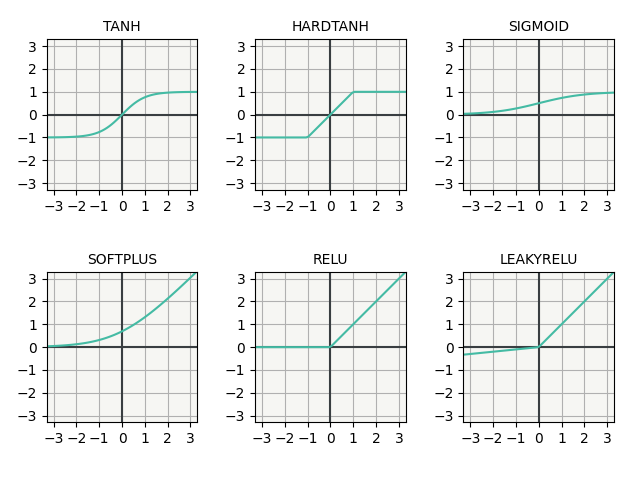
\includegraphics[width=6in]{../cap1_preliminares/src/activations.png}
        \caption{Funciones de activación comunmente utilizadas}
    \end{figure}
    
    % Transferemcia de aprendizaje
    \subsection{Transferencia de aprendizaje}
    La transferencia de aprendizaje en el campo del aprendizaje profundo, es un concepto motivado por la psicología, que se basa en usar conocimientos adquiridos para cierta tarea $A$, con el objetivo de aprender alguna tarea $B$ \cite{transfer}. Por ejemplo, si una persona sabe bailar salsa, posiblemente pueda usar esos conocimientos para aprender a bailar bachata. 

    En la mayoría de los casos, los conjuntos de datos tienen una cantidad limitada de imágenes etiquetadas. Una posible solución a este problema, es usar \textsl{aprendizaje semisupervisado}, el cuál requiere algunas imágenes etiquetadas, pero también se pueden usar varias imágenes no etiquetadas. Sin embargo, incluso los conjuntos de datos no etiquetados, pueden ser insuficientes. Cuando se tienen conjuntos de datos muy pequeños, es posible apoyarse de modelos pre-entrenados con millones de imágenes, con la esperanza de que las características aprendidas anteriormente, sean de utilidad en el nuevo conjunto de datos.
    % Conjuntos desbalanceados
    \subsection{Conjuntos desbalanceados} 
    \label{unbalanced_sets}
    Cuando se enfrenta el problema de clasificación, digamos con $m$ clases, uno esperaría que tengamos suficientes ejemplos de cada clase. Más aún, para que nuestro modelo no tenga ningún sesgo por ninguna clase, es preferible que en nuestro conjunto de entrenamiento, todas las clases tengan una cantidad similar de ejemplos. De lo contrario, nuestro modelo podría ser entrenado con demasiados elementos de una clase particular $\mathcal C$, y tendería a clasificar muchos elementos en la clase $\mathcal C$. Además de esto, si nuestro conjunto de prueba también está desbalanceado, no se vería reflejado el sesgo en métricas comunes como la exactitud y la precisión.

    \begin{definition}
    \label{balanced}
        Sea $\mathcal C$ un conjunto de datos, cuyas clases son $\mathcal C_1, ..., \mathcal C_m$. Un conjunto de datos se dice balanceado con tolerancia de $\epsilon$ si 
        \begin{equation}
            1-\epsilon \leq \frac{|C_i|}{|C_j|} \leq 1 + \epsilon, \quad i,j = 1,2, ..., m.
        \end{equation}
        Un conjunto es desbalanceado bajo la tolerancia $\epsilon$ si no es balanceado.
    \end{definition}
    Para efectos prácticos, diremos que un conjunto balanceado con tolerancia $\epsilon = 0.1$
    \begin{example}
        Supóngase ahora que dada una lista de características, se quiere clasificar a las personas infectadas de COVID-19. En México el índice de positividad en la semana 46 fue del $17\%$ \cite{grafica}. Por lo que si se toman todas las pruebas realizadas se tendría la siguiente razón:
        \begin{equation}
            \frac{|C_{Neg}|}{|C_{Pos}|} = 4.8823 > 1.1.
        \end{equation}
        El tamaño de la clase de pruebas negativas es casi 5 veces mayor al tamaño de la clase de pruebas positivas. Por consiguiente, estaríamos en presencia de un conjunto de datos desbalanceado.
    \end{example}
    \begin{figure}[H]
        \centering
        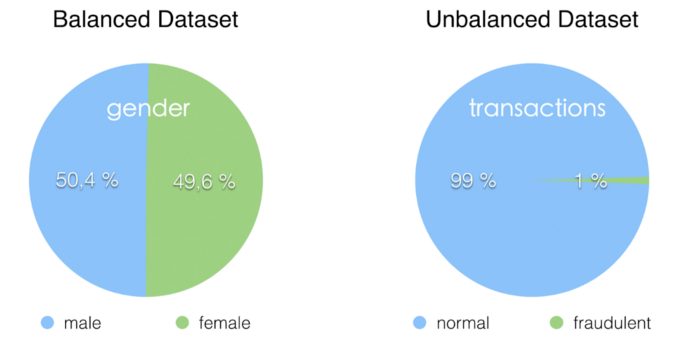
\includegraphics[width=6in]{../cap1_preliminares/src/unbalanced.png}
        \caption{Ejemplos de conjuntos balanceados y desbalanceados.}
    \end{figure}
    \subsubsection{Afrontar un problema con un conjunto desbalanceado}
    La forma principal de lidiar con un conjunto desbalanceado es, valga la redundancia \textsl{balancear el conjunto}. Es decir, forzar al conjunto a tener clases cuyos tamaños coincidan. Para conseguir esto, es posible seguir distintas estrategias.
    \begin{itemize}
        \item \textbf{Submuestreo.} Consiste en tomar la clase mayoritaria (la clase con menor número de elementos) y eliminar algunas instancias, de modo que el conjunto quede balanceado. La manera más sencilla, es tomando elementos aleatorios del conjunto. Sin embargo, esto puede retirar instancias que contengan información esencial, por lo que sólo es recomendable en caso de tener un conjunto de datos muy grande.

        Otros algoritmos, heurísticos se basan en dos diferentes modelos de teoría de ruido. Algunos investigadores consideran que las instancias cercanas a los márgenes de clasificación de dos clases, son consideradas ruido. Por otro lado, algunos investigadores consideran que las instancias presentes en vecindades de varias etiquetas distintas, se pueden considerar como ruido. De modo que en lugar de remover elementos aleatorios, estas estrategias implican hacer el submuestreo tomando en cuenta únicamente las instancias que no sean ruido.

        \item \textbf{Sobremuestreo.} Al igual que en el submuestreo, existe el sobremuestreo aleatorio, el cual se basa en crear copias idénticas de las instancias de la clase minoritaria, de modo que la nuestra clase minoritaria alcance la magnitud del resto de clases. Al aplicar este método, se incrementa el riesgo de sobreajustar el modelo. 

        Otros algoritmos de sobremuestreo, generan instancias sintéticas para incrementar la cantidad de datos en una clase. Existen diversas formas de conseguir esto. Una posibilidad, es usando el aumento de datos únicamente en la clase minoritaria, permitiendo rotaciones, traslaciones y otras transformaciones. Existe también algoritmos como el VAE \cite{VAE}, SMOTE \cite{SMOTE}, MSMOTE \cite{MSMOTE}. 

    \end{itemize}

    \begin{figure}[H]
        \centering
        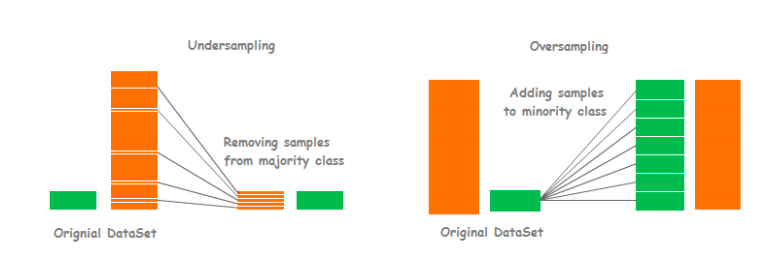
\includegraphics[width=6in]{../cap1_preliminares/src/undersampling_oversampling.png}
        \caption{Representación gráfica del submuestreo y el sobremuestreo.}
    \end{figure}

    \subsubsection{Métricas distintas a la exactitud}
    Como hemos mencionado antes, la exactitud no debe ser la única métrica a considerar en un problema con conjunto de datos desbalanceado. La razón es simple: es posible obtener una muy buena exactitud sin realmente hacer predicciones de nuestra clase minoritaria.
    \begin{example}
        \label{diff_metrics}
        Si tenemos un conjunto de datos con dos clases, tal que una clase $C_1$ representa el $99\%$ de las instancias, y la clase $C_2$ el $1\%$ restante. Si tomamos el clasificador $f: \mathcal C \to \{1,2\}$, $f(x) = 1$. Claramente nuestra exactitud sería del $99\%$, pero las predicciones de nuestra clase minoritaria aciertan un $0\%$ de las veces.
    \end{example}{}
    Una forma de sobrellevar el efecto visto en el ejemplo \ref{diff_metrics} es analizando el desempeño del clasificador para cada clase por separado y luego hacer un promedio. En el caso de nuestro ejemplo todas las instancias que en verdad pertenecen a la clase 1, fueron clasificadas correctamente (1.0), y las instancias que pertenecen a la clase 2, fueron clasificadas todas incorrectamente (0.0). Con lo con esta nueva métrica tendríamos una puntuación de $\frac{1.0 + 0.0}{2} = 0.5$. En el capítulo \ref{experimentos} se definen formalmente las métricas relevantes para este trabajo. Sin embargo, las métricas más utilizadas para este tipo de problemas son las siguientes:
    \begin{itemize}
        \item Confussion matrix: De ésta matriz, se pueden obtener métricas útiles tales como Especificidad, Sensitividad, Precisión, Recall
        \item F1-score: La media armónica de precisión
         y recall
        \item ROC curves
        \item Logloss
        \item Kappa: Exactitud de la clasificación, normalizada por el desbalance de clases en nuestros datos.
    \end{itemize}
